\emph{If you want to get involved, write to
\href{http://en.wikipedia.org/wiki/Howard_Rheingold}{Howard Rheingold}
at \href{mailto:howard@rheingold.com}{howard@rheingold.com}.}

\subsection{Hello and welcome!}

The peeragogy project was kicked off around the time of
\href{http://rheingold.com/}{Howard Rheingold's} January 23,
2012~\href{http://vimeo.com/35685124}{Regents Lecture} at UC Berkeley on
\emph{Social Media and Peer Learning: From Mediated Pedagogy to
Peeragogy}.~ We have put together a handbook about peer learning: you're
reading it -- maybe on \href{peeragogy.org}{our website}, or in your
hammock with the beverage of your choice and our
\href{http://www.lulu.com/shop/howard-rheingold-and-peeragogyorg-editors/the-peeragogy-handbook/paperback/product-20607425.html}{print
on demand} paperback.~ Or maybe you grabbed our
\href{http://peeragogy.net/peeragogy-handbook-v1-1.pdf}{free PDF} or
some other remixed version in some other format or flavor from some
other place (which would be
\href{http://peeragogy.org/resources/license/}{cool}!).

But: there's still
\href{http://peeragogy.org/peeragogy-org-roadmap/}{more work to be
done}.~ We created this page because you might be interested in getting
involved in improving the book or furthering the project in other ways.~
If so, we're happy to have you aboard!

What you do here is largely up to you.~ Asking questions is actually
extremely helpful: there's almost always someone in our
\href{https://plus.google.com/u/0/communities/107386162349686249470}{Google+
community} who would be happy to try to answer them, or refer you to
someone else who can. Or just poke around the public pages on
peeragogy.org and leave a comment or two.~ Better still, find an area
where you feel knowledgeable -- or are willing to learn -- and start
writing (or filming, dancing, drawing, building, etc.).
The goal we have in mind for our book is for it be a useful guide to
peer learning! To achieve that goal we have in mind multiple
opportunities for peers to contribute.~ Here's our current ``Top Ten''
list:

\href{http://peeragogy.org/wp-content/uploads/2012/03/what_to_do_color.gif}{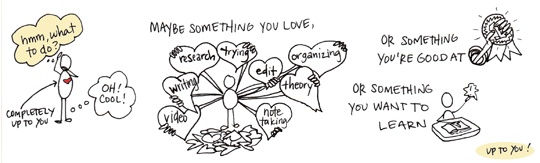
\includegraphics{http://peeragogy.org/wp-content/uploads/2012/03/what_to_do_color.gif}}

\begin{enumerate}
\item
  \begin{itemize}
  \itemsep1pt\parskip0pt\parsep0pt
  \item
    Site: Peeragogy.org
  \item
    What happens: Maintain the ``master'' copy of the peeragogy
    handbook, public new about the project
  \item
    Who's in charge: Peeragogy Editorial Board, Stephanie Schipper,
    Howard Rheingold
  \item
    URL: \href{http://peeragogy.org}{http://peeragogy.org}
  \item
    Status: Active
  \end{itemize}
\item
  \begin{itemize}
  \itemsep1pt\parskip0pt\parsep0pt
  \item
    Site: Google Docs
  \item
    What happens: Hive editing, working drafts to be delivered elsewhere
    when they are finished or for final polishing
  \item
    Who's in charge: Everyone
  \item
    URL: \href{https://drive.google.com}{https://drive.google.com}
  \item
    Status: Active
  \end{itemize}
\item
  \begin{itemize}
  \itemsep1pt\parskip0pt\parsep0pt
  \item
    Site: PIA Google+
  \item
    What happens: Random posts related to Peeragogy, quick
    communications between members, news about events, hangouts, etc
  \item
    Who's in charge: Everyone
  \item
    URL: \href{http://goo.gl/4dRU92}{http://goo.gl/4dRU92}
  \item
    Status: Active
  \end{itemize}
\item
  \begin{itemize}
  \itemsep1pt\parskip0pt\parsep0pt
  \item
    Site: +Peeragogy Handbook page
  \item
    What happens: Coordinating Hangouts on Air, G+ news updates
  \item
    Who's in charge: Charlotte Pierce
  \item
    URL:
    \href{https://plus.google.com/+PeeragogyOrgHandbook/posts}{https://plus.google.com/+PeeragogyOrgHandbook/posts}
  \item
    Status: Active
  \end{itemize}
\item
  \begin{itemize}
  \itemsep1pt\parskip0pt\parsep0pt
  \item
    Site: Peeragogy YouTube Channel
  \item
    What happens: videos posted here
  \item
    Who's in charge: Charlotte Pierce
  \item
    URL:
    \href{http://www.youtube.com/channel/UCAQ5TpUxKrsVfWtIHMaDh5A/about}{http://www.youtube.com/channel/UCAQ5TpUxKrsVfWtIHMaDh5A/}
  \item
    Status: Active
  \end{itemize}
\item
  \begin{itemize}
  \itemsep1pt\parskip0pt\parsep0pt
  \item
    Site: Commons Abundance Network
  \item
    What happens: Public facing landing page for the accelerator,
    networking with other commons-oriented groups
  \item
    Who's in charge: Helene Finidori
  \item
    URL:
    \href{http://commonsabundance.net/groups/peeragogy/}{http://commonsabundance.net/groups/peeragogy/}
  \item
    Status: Active
  \end{itemize}
\item
  \begin{itemize}
  \itemsep1pt\parskip0pt\parsep0pt
  \item
    Site: PPT Google+
  \item
    What happens: Meta-level coordination for the project
  \item
    Who's in charge: Peeragogy Editorial Board
  \item
    URL: \href{http://goo.gl/AzxXQq}{http://goo.gl/AzxXQq}
  \item
    Status: Active
  \end{itemize}
\item
  \begin{itemize}
  \itemsep1pt\parskip0pt\parsep0pt
  \item
    Site: Git.io/Handbook
  \item
    What happens: versioned storage of the LaTeX sources for the print
    version of the handbook and other derived formats and scripts
  \item
    Who's in charge: Joe Corneli
  \item
    URL: \href{http://git.io/Handbook}{http://git.io/Handbook}
  \item
    Status: Low traffic
  \end{itemize}
\item
  \begin{itemize}
  \itemsep1pt\parskip0pt\parsep0pt
  \item
    Site: Peeragogy mailing list
  \item
    What happens: Meta-level coordination for the project, main point of
    contact with the email-o-sphere
  \item
    Who's in charge: Joe Corneli
  \item
    URL:
    \href{https://groups.google.com/forum/\#!forum/peeragogy}{https://groups.google.com/forum/\#!forum/peeragogy}
  \item
    Status: Low traffic
  \end{itemize}
\item
  \begin{itemize}
  \itemsep1pt\parskip0pt\parsep0pt
  \item
    Site: Paragogy.net
  \item
    What happens: Wiki editing if and when that makes sense, e.g.~for
    translations or large multi-part documents
  \item
    Who's in charge: Joe Corneli, Charlie Danoff, Fabrizio Terzi
  \item
    URL: \href{http://paragogy.net}{http://paragogy.net}
  \item
    Status: Low traffic
  \end{itemize}
\end{enumerate}

It's up to you. Instead of worrying too much about
\href{http://peeragogy.org/co-working/}{the rules}, or trying to master
all of the \href{http://peeragogy.org/resources/technologies/}{tools we
use} at all once, you can just jump in by joining our conversations, and
take advantage of the digital memory of the forum to rewind the
conversation all the way to the beginning (if you want to go that far),
listen in for a little bit if you want to, and jump in whenever you're
ready.~ There are always lots of things to do (including many that no
one here has thought of yet).~ We won't know what you're up to until you
speak up. You can have a look at the outstanding tasks and teams that
are listed on
\href{https://docs.google.com/document/d/1_2I-z-Pt5NUKk-fpy4jsqxFeXbWS4ao4sIhkxCcRVeI/edit\#}{this
Google Doc}: our
\href{http://peeragogy.org/peeragogy-org-roadmap/}{roadmap} is a useful
shared resource too.~ You can add to these at any time.

We regularly use Google+, Google Hangouts, forums, and email to
communicate asynchronously and pretty much continuously. We also meet
irregularly as a group for synchronous audio-video sessions. Further
details about all these methods of communication can be found below.

In short: here's how it works:

\href{http://peeragogy.org/wp-content/uploads/2012/03/lots_going_on_color_1000.gif}{\includegraphics{http://peeragogy.org/wp-content/uploads/2012/03/lots_going_on_color_1000-e1352754548930.gif}}
~
\href{http://peeragogy.org/wp-content/uploads/2012/03/where_to_go_color.gif}{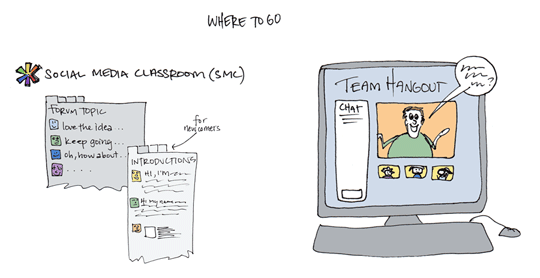
\includegraphics{http://peeragogy.org/wp-content/uploads/2012/03/where_to_go_color.gif}}

%\section{\textbf{\href{http://peeragogy.org/wp-content/uploads/2012/03/create_content.gif}{\includegraphics{http://peeragogy.org/wp-content/uploads/2012/03/create_content-300x145.gif}}}}

~
\textbf{\href{http://peeragogy.org/wp-content/uploads/2012/03/communicate_color1.gif}{\includegraphics{http://peeragogy.org/wp-content/uploads/2012/03/communicate_color1-300x67.gif}}}
\textbf{~
\href{http://peeragogy.org/wp-content/uploads/2012/03/questions_1000.gif}{\includegraphics{http://peeragogy.org/wp-content/uploads/2012/03/questions_1000-300x50.gif}}}

\subsection{Questions?}

If you have questions, that's good!~ Use Google+ or post a comment on
peeragogy.org, email the team energy center if you know who that is, or
email~\href{mailto:howard@rheingold.com}{howard@rheingold.com}.
